\documentclass{extbook}[14pt]
\usepackage{multicol, enumerate, enumitem, hyperref, color, soul, setspace, parskip, fancyhdr, amssymb, amsthm, amsmath, latexsym, units, mathtools}
\everymath{\displaystyle}
\usepackage[headsep=0.5cm,headheight=0cm, left=1 in,right= 1 in,top= 1 in,bottom= 1 in]{geometry}
\usepackage{dashrule}  % Package to use the command below to create lines between items
\newcommand{\litem}[1]{\item #1

\rule{\textwidth}{0.4pt}}
\pagestyle{fancy}
\lhead{}
\chead{Answer Key for Progress Quiz 6 Version C}
\rhead{}
\lfoot{1430-1829}
\cfoot{}
\rfoot{test}
\begin{document}
\textbf{This key should allow you to understand why you choose the option you did (beyond just getting a question right or wrong). \href{https://xronos.clas.ufl.edu/mac1105spring2020/courseDescriptionAndMisc/Exams/LearningFromResults}{More instructions on how to use this key can be found here}.}

\textbf{If you have a suggestion to make the keys better, \href{https://forms.gle/CZkbZmPbC9XALEE88}{please fill out the short survey here}.}

\textit{Note: This key is auto-generated and may contain issues and/or errors. The keys are reviewed after each exam to ensure grading is done accurately. If there are issues (like duplicate options), they are noted in the offline gradebook. The keys are a work-in-progress to give students as many resources to improve as possible.}

\rule{\textwidth}{0.4pt}

\begin{enumerate}\litem{
Write the equation of the graph presented below in the form $f(x)=ax^2+bx+c$, assuming  $a=1$ or $a=-1$. Then, choose the intervals that $a, b,$ and $c$ belong to.

\begin{center}
    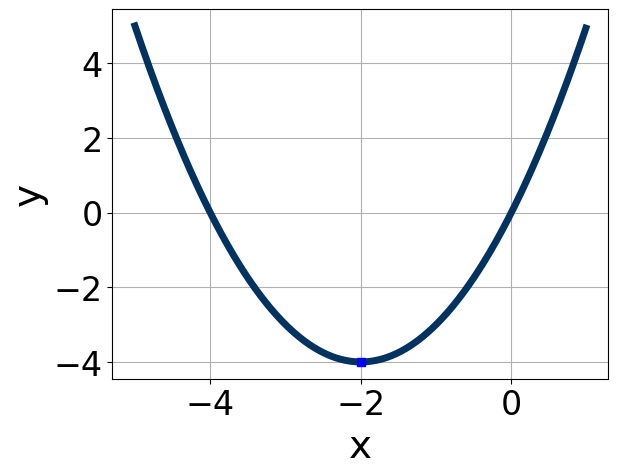
\includegraphics[width=0.5\textwidth]{../Figures/quadraticGraphToEquationCopyC.png}
\end{center}


The solution is \( f(x) = x^{2} -4 x -2 \), which is option B.\begin{enumerate}[label=\Alph*.]
\item \( a \in [0, 1.9], \hspace*{5mm} b \in [0, 9], \text{ and } \hspace*{5mm} c \in [10, 11] \)

$f(x)=x^{2} +4 x + 10$, which corresponds to incorrectly using vertex form as $f(x) = a(x+h)^2 - k$.
\item \( a \in [0, 1.9], \hspace*{5mm} b \in [-7, -3], \text{ and } \hspace*{5mm} c \in [-2, 2] \)

* $f(x)=x^{2} -4 x -2$, which is the correct option.
\item \( a \in [0, 1.9], \hspace*{5mm} b \in [0, 9], \text{ and } \hspace*{5mm} c \in [-2, 2] \)

$f(x)=x^{2} +4 x -2$, which corresponds to incorrectly using vertex form as $f(x) = a(x+h)^2+k$.
\item \( a \in [-2.3, -0.6], \hspace*{5mm} b \in [0, 9], \text{ and } \hspace*{5mm} c \in [-12, -9] \)

$f(x)=-x^{2} +4 x -10$, which corresponds to making $a$ the opposite sign than it should be.
\item \( a \in [-2.3, -0.6], \hspace*{5mm} b \in [-7, -3], \text{ and } \hspace*{5mm} c \in [-12, -9] \)

$f(x)=-x^{2} -4 x -10$, which corresponds to incorrectly using vertex form as $f(x) = a(x+h)^2+k$ AND making $a$ the opposite sign than it should be.
\end{enumerate}

\textbf{General Comment:} When the graph is pointing up, $a=1$. When the graph is pointing down, $a=-1$. Be sure to use Vertex Form: $y = a(x-h)^2+k$.
}
\litem{
Factor the quadratic below. Then, choose the intervals that contain the constants in the form $(ax+b)(cx+d); b \leq d.$
\[ 24x^{2} +50 x + 25 \]The solution is \( (4x + 5)(6x + 5) \), which is option A.\begin{enumerate}[label=\Alph*.]
\item \( a \in [3.59, 5.5], \hspace*{5mm} b \in [4, 11], \hspace*{5mm} c \in [5.91, 6.34], \text{ and } \hspace*{5mm} d \in [1, 6] \)

* $(4x + 5)(6x + 5)$, which is the correct option.
\item \( a \in [1.68, 3.64], \hspace*{5mm} b \in [4, 11], \hspace*{5mm} c \in [11.87, 12.15], \text{ and } \hspace*{5mm} d \in [1, 6] \)

 $(2x + 5)(12x + 5)$, which corresponds to associating some factor of c to a.
\item \( a \in [-1.04, 1.56], \hspace*{5mm} b \in [17, 26], \hspace*{5mm} c \in [0.92, 1.21], \text{ and } \hspace*{5mm} d \in [23, 33] \)

 $(x + 20)(x + 30)$, which corresponds to factoring $x^{2} +50 x + 600$.
\item \( a \in [11.73, 13.03], \hspace*{5mm} b \in [4, 11], \hspace*{5mm} c \in [1.2, 2.99], \text{ and } \hspace*{5mm} d \in [1, 6] \)

 $(12x + 5)(2x + 5)$, which corresponds to associating some factor of a to c.
\item \( \text{None of the above.} \)

 Corresponds to a different factoring than any of the predicted options. If you get this, please let the coordinator know so they can work with you to figure out what went wrong with your factoring.
\end{enumerate}

\textbf{General Comment:} $ac$ had many factors in this problem. It is best to list out the possible pairs in order to make sure you don't miss any.
}
\litem{
Solve the quadratic equation below. Then, choose the intervals that the solutions $x_1$ and $x_2$ belong to, with $x_1 \leq x_2$.
\[ 15x^{2} +2 x -24 = 0 \]The solution is \( x_1 = -1.333 \text{ and } x_2 = 1.200 \), which is option E.\begin{enumerate}[label=\Alph*.]
\item \( x_1 \in [-0.84, 0.34] \text{ and } x_2 \in [2.23, 2.89] \)

$x_1 = -0.667 \text{ and } x_2 = 2.400$, which corresponds to solving the factored version $(3x + 2)(5x -12)$
\item \( x_1 \in [-20.64, -19.82] \text{ and } x_2 \in [17.81, 18.57] \)

$x_1 = -20.000 \text{ and } x_2 = 18.000$, which corresponds to solving the factored version $(x + 20)(x -18)$
\item \( x_1 \in [-2.86, -1.67] \text{ and } x_2 \in [0.52, 0.81] \)

$x_1 = -2.667 \text{ and } x_2 = 0.600$, which corresponds to solving the factored version $(3x + 8)(5x -3)$
\item \( x_1 \in [-4.09, -3.97] \text{ and } x_2 \in [0.35, 0.45] \)

$x_1 = -4.000 \text{ and } x_2 = 0.400$, which corresponds to solving the factored version $(x + 4)(15x -6)$
\item \( x_1 \in [-1.46, -0.8] \text{ and } x_2 \in [1.17, 1.62] \)

* $x_1 = -1.333 \text{ and } x_2 = 1.200$, which is the correct option. Obtained by solving the factored version $(3x + 4)(5x -6)$
\end{enumerate}

\textbf{General Comment:} This question can be factored, but it may be faster to find the solutions via the Quadratic Equation.
}
\litem{
Graph the equation below.
\[ f(x) = (x+2)^2 + 13 \]The solution is the graph below, which is option D.
\begin{center}
    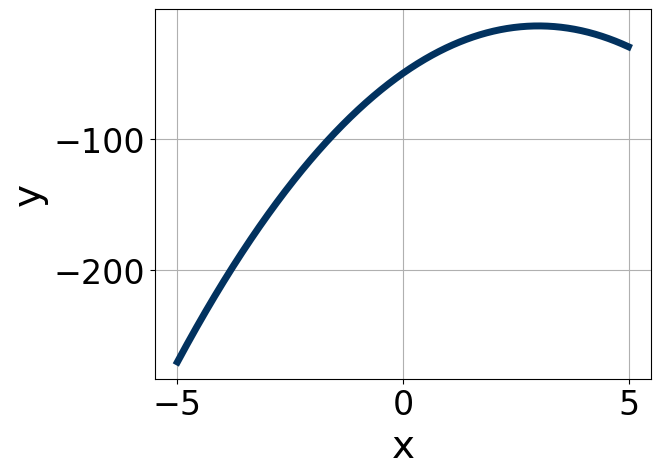
\includegraphics[width=0.3\textwidth]{../Figures/quadraticEquationToGraphCopyDC.png}
\end{center}\begin{enumerate}[label=\Alph*.]
\begin{multicols}{2}
\item 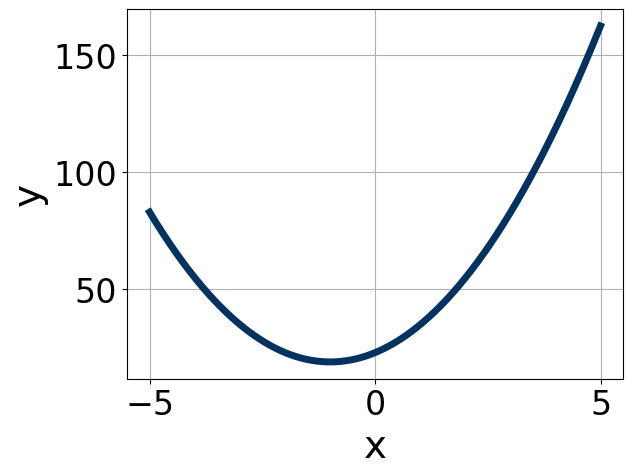
\includegraphics[width = 0.3\textwidth]{../Figures/quadraticEquationToGraphCopyAC.png}
\item 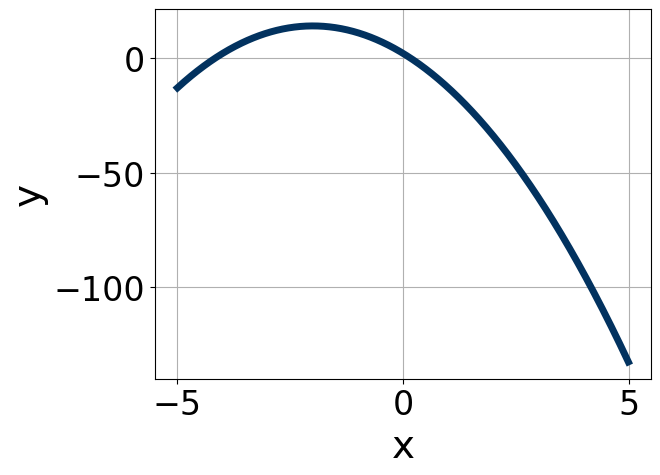
\includegraphics[width = 0.3\textwidth]{../Figures/quadraticEquationToGraphCopyBC.png}
\item 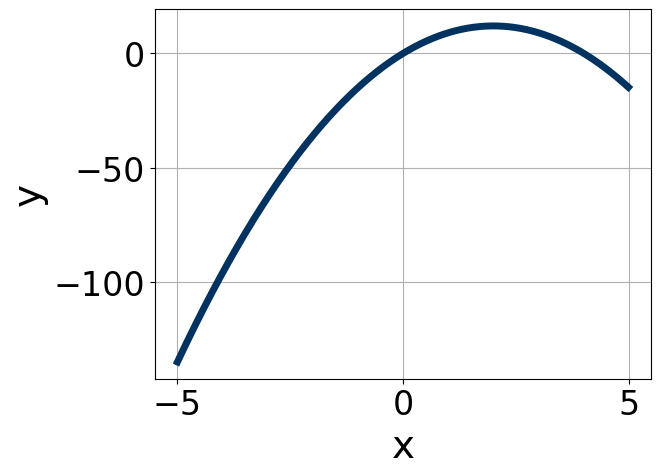
\includegraphics[width = 0.3\textwidth]{../Figures/quadraticEquationToGraphCopyCC.png}
\item 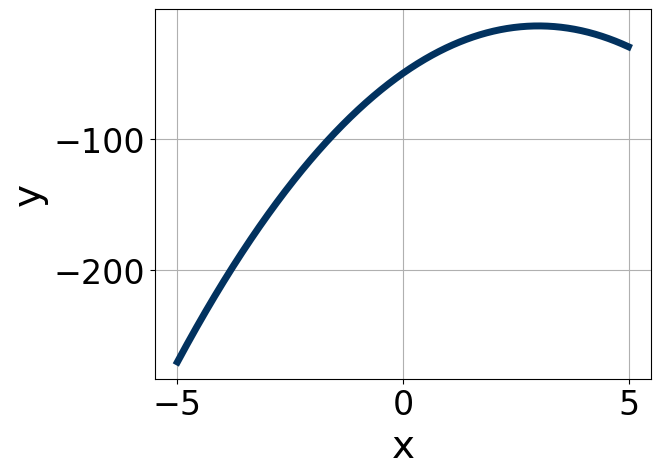
\includegraphics[width = 0.3\textwidth]{../Figures/quadraticEquationToGraphCopyDC.png}
\end{multicols}\item None of the above.\end{enumerate}
\textbf{General Comment:} Remember that Vertex Form is $y = a(x-h)^2+k$, where the vertex is $(h, k)$.
}
\litem{
Graph the equation below.
\[ f(x) = (x-1)^2 - 10 \]The solution is the graph below, which is option D.
\begin{center}
    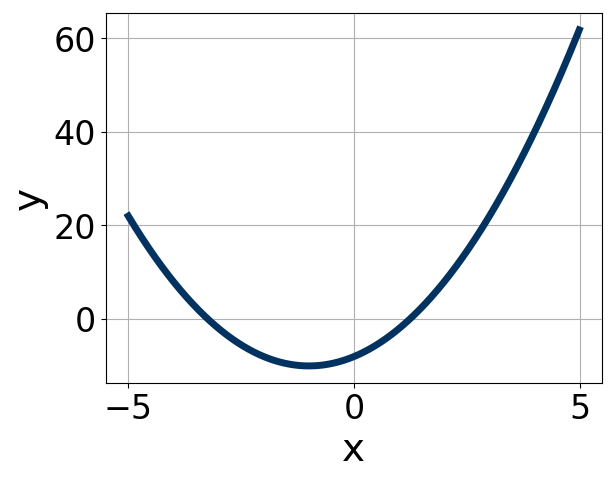
\includegraphics[width=0.3\textwidth]{../Figures/quadraticEquationToGraphDC.png}
\end{center}\begin{enumerate}[label=\Alph*.]
\begin{multicols}{2}
\item 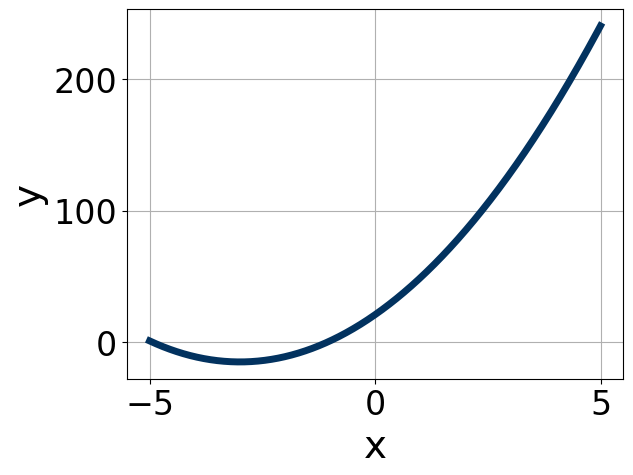
\includegraphics[width = 0.3\textwidth]{../Figures/quadraticEquationToGraphAC.png}
\item 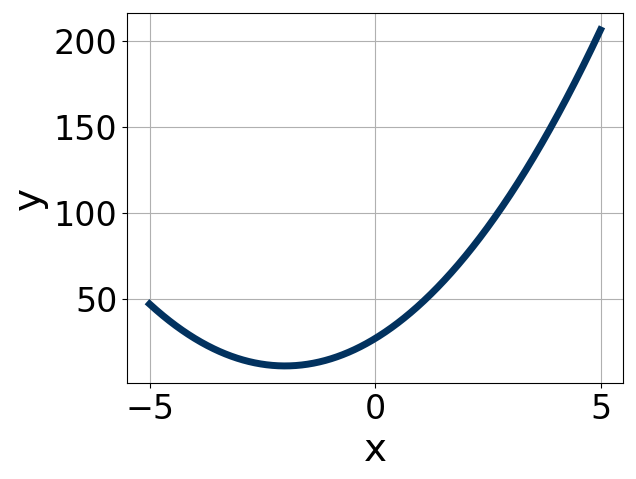
\includegraphics[width = 0.3\textwidth]{../Figures/quadraticEquationToGraphBC.png}
\item 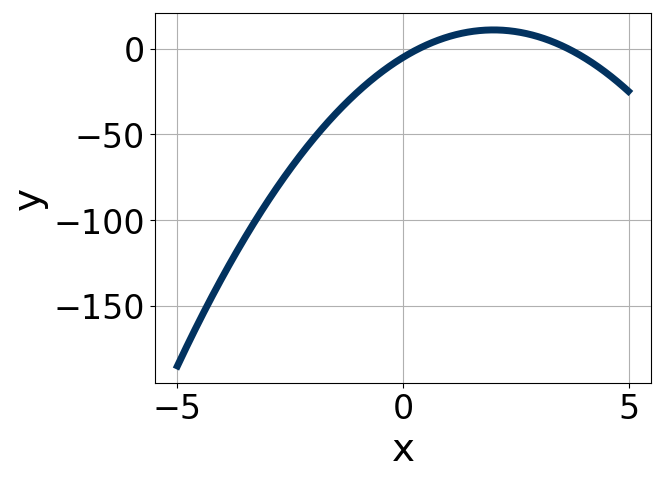
\includegraphics[width = 0.3\textwidth]{../Figures/quadraticEquationToGraphCC.png}
\item 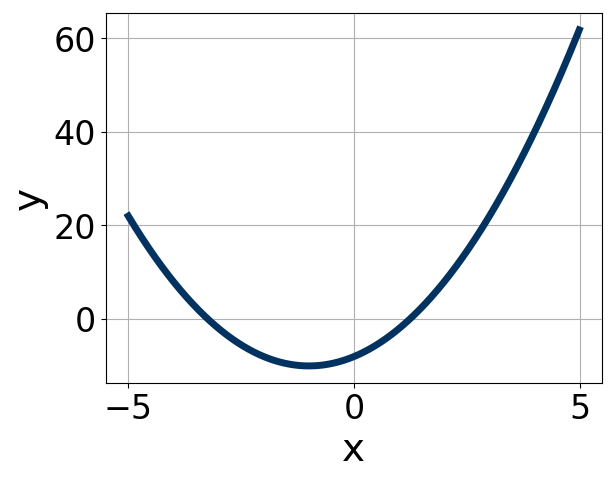
\includegraphics[width = 0.3\textwidth]{../Figures/quadraticEquationToGraphDC.png}
\end{multicols}\item None of the above.\end{enumerate}
\textbf{General Comment:} Remember that Vertex Form is $y = a(x-h)^2+k$, where the vertex is $(h, k)$.
}
\litem{
Write the equation of the graph presented below in the form $f(x)=ax^2+bx+c$, assuming  $a=1$ or $a=-1$. Then, choose the intervals that $a, b,$ and $c$ belong to.

\begin{center}
    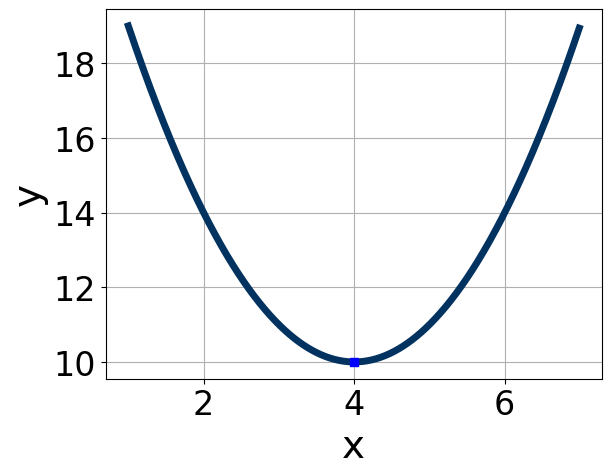
\includegraphics[width=0.5\textwidth]{../Figures/quadraticGraphToEquationC.png}
\end{center}


The solution is \( f(x) = -x^{2} +8 x -20 \), which is option E.\begin{enumerate}[label=\Alph*.]
\item \( a \in [1, 5], \hspace*{5mm} b \in [-9, -7], \text{ and } \hspace*{5mm} c \in [9, 14] \)

$f(x)=x^{2} -8 x + 12$, which corresponds to making $a$ the opposite sign than it should be.
\item \( a \in [1, 5], \hspace*{5mm} b \in [6, 12], \text{ and } \hspace*{5mm} c \in [9, 14] \)

$f(x)=x^{2} +8 x + 12$, which corresponds to incorrectly using vertex form as $f(x) = a(x+h)^2+k$ AND making $a$ the opposite sign than it should be.
\item \( a \in [-3, 0], \hspace*{5mm} b \in [-9, -7], \text{ and } \hspace*{5mm} c \in [-13, -11] \)

$f(x)=-x^{2} -8 x -12$, which corresponds to incorrectly using vertex form as $f(x) = a(x+h)^2 - k$.
\item \( a \in [-3, 0], \hspace*{5mm} b \in [-9, -7], \text{ and } \hspace*{5mm} c \in [-22, -19] \)

$f(x)=-x^{2} -8 x -20$, which corresponds to incorrectly using vertex form as $f(x) = a(x+h)^2+k$.
\item \( a \in [-3, 0], \hspace*{5mm} b \in [6, 12], \text{ and } \hspace*{5mm} c \in [-22, -19] \)

* $f(x)=-x^{2} +8 x -20$, which is the correct option.
\end{enumerate}

\textbf{General Comment:} When the graph is pointing up, $a=1$. When the graph is pointing down, $a=-1$. Be sure to use Vertex Form: $y = a(x-h)^2+k$.
}
\litem{
Solve the quadratic equation below. Then, choose the intervals that the solutions $x_1$ and $x_2$ belong to, with $x_1 \leq x_2$.
\[ 25x^{2} -60 x + 36 = 0 \]The solution is \( x_1 = 1.200 \text{ and } x_2 = 1.200 \), which is option A.\begin{enumerate}[label=\Alph*.]
\item \( x_1 \in [1.2, 1.28] \text{ and } x_2 \in [0.02, 2.18] \)

* $x_1 = 1.200 \text{ and } x_2 = 1.200$, which is the correct option. Obtained by solving the factored version $(5x -6)(5x -6)$
\item \( x_1 \in [29.84, 30.02] \text{ and } x_2 \in [29.27, 30.72] \)

$x_1 = 30.000 \text{ and } x_2 = 30.000$, which corresponds to solving the factored version $(x -30)(x -30)$
\item \( x_1 \in [0.51, 0.68] \text{ and } x_2 \in [2.07, 2.53] \)

$x_1 = 0.600 \text{ and } x_2 = 2.400$, which corresponds to solving the factored version $(5x -3)(5x -12)$
\item \( x_1 \in [0.22, 0.28] \text{ and } x_2 \in [5.71, 6.33] \)

$x_1 = 0.240 \text{ and } x_2 = 6.000$, which corresponds to solving the factored version $(25x -6)(x -6)$
\item \( x_1 \in [0.32, 0.41] \text{ and } x_2 \in [2.97, 4.3] \)

$x_1 = 0.400 \text{ and } x_2 = 3.600$, which corresponds to solving the factored version $(5x -2)(5x -18)$
\end{enumerate}

\textbf{General Comment:} This question can be factored, but it may be faster to find the solutions via the Quadratic Equation.
}
\litem{
Factor the quadratic below. Then, choose the intervals that contain the constants in the form $(ax+b)(cx+d); b \leq d.$
\[ 36x^{2} +43 x + 12 \]The solution is \( (4x + 3)(9x + 4) \), which is option D.\begin{enumerate}[label=\Alph*.]
\item \( a \in [-0.7, 1.2], \hspace*{5mm} b \in [15, 19], \hspace*{5mm} c \in [-4.7, 3.3], \text{ and } \hspace*{5mm} d \in [23, 28] \)

 $(x + 16)(x + 27)$, which corresponds to factoring $x^{2} +43 x + 432$.
\item \( a \in [-0.7, 1.2], \hspace*{5mm} b \in [-3, 10], \hspace*{5mm} c \in [24.8, 30.7], \text{ and } \hspace*{5mm} d \in [0, 7] \)

 $(x + 3)(27x + 4)$, which corresponds to associating some factor of c to a.
\item \( a \in [5.6, 10.6], \hspace*{5mm} b \in [-3, 10], \hspace*{5mm} c \in [3.3, 5.9], \text{ and } \hspace*{5mm} d \in [0, 7] \)

 $(8x + 3)(4x + 4)$, which corresponds to associating some factor of a to c.
\item \( a \in [2.1, 5.6], \hspace*{5mm} b \in [-3, 10], \hspace*{5mm} c \in [8.8, 10.7], \text{ and } \hspace*{5mm} d \in [0, 7] \)

* $(4x + 3)(9x + 4)$, which is the correct option.
\item \( \text{None of the above.} \)

 Corresponds to a different factoring than any of the predicted options. If you get this, please let the coordinator know so they can work with you to figure out what went wrong with your factoring.
\end{enumerate}

\textbf{General Comment:} $ac$ had many factors in this problem. It is best to list out the possible pairs in order to make sure you don't miss any.
}
\litem{
Solve the quadratic equation below. Then, choose the intervals that the solutions belong to, with $x_1 \leq x_2$ (if they exist).
\[ 16x^{2} +13 x -6 = 0 \]The solution is \( x_1 = -1.141 \text{ and } x_2 = 0.329 \), which is option D.\begin{enumerate}[label=\Alph*.]
\item \( x_1 \in [-21.2, -17.8] \text{ and } x_2 \in [5, 6.1] \)

 $x_1 = -18.258 \text{ and } x_2 = 5.258$, which corresponds to using the Quadratic Formula with $a=1$
\item \( x_1 \in [-25.3, -23.6] \text{ and } x_2 \in [22.2, 25.4] \)

 $x_1 = -23.922 \text{ and } x_2 = 23.110$, which corresponds to writing the Quadratic Formula as $-\frac{b}{2a} \pm \sqrt{b^2 - 4ac}$.
\item \( x_1 \in [-1.1, 1] \text{ and } x_2 \in [0.6, 2.2] \)

 $x_1 = -0.329 \text{ and } x_2 = 1.141$, which corresponds to writing the Quadratic Formula as $\frac{b \pm \sqrt{b^2 - 4ac}}{2a}$
\item \( x_1 \in [-1.3, -0.6] \text{ and } x_2 \in [-0.1, 0.4] \)

* $x_1 = -1.141 \text{ and } x_2 = 0.329$, which is the correct option.
\item \( \text{There are no Real solutions.} \)

Corresponds to getting a negative under the radical or believing that since the quadratic cannot be factored, it has no Real solutions.
\end{enumerate}

\textbf{General Comment:} This requires Quadratic Formula. Just be sure to use the correct formula and watch your signs.
}
\litem{
Solve the quadratic equation below. Then, choose the intervals that the solutions belong to, with $x_1 \leq x_2$ (if they exist).
\[ -11x^{2} +7 x + 6 = 0 \]The solution is \( x_1 = -0.486 \text{ and } x_2 = 1.122 \), which is option C.\begin{enumerate}[label=\Alph*.]
\item \( x_1 \in [-17.74, -16.31] \text{ and } x_2 \in [17.57, 18.71] \)

 $x_1 = -17.374 \text{ and } x_2 = 18.010$, which corresponds to writing the Quadratic Formula as $-\frac{b}{2a} \pm \sqrt{b^2 - 4ac}$.
\item \( x_1 \in [-12.67, -12.24] \text{ and } x_2 \in [5.23, 5.44] \)

 $x_1 = -12.346 \text{ and } x_2 = 5.346$, which corresponds to using the Quadratic Formula with $a=1$
\item \( x_1 \in [-1.02, 0.29] \text{ and } x_2 \in [0.74, 1.56] \)

* $x_1 = -0.486 \text{ and } x_2 = 1.122$, which is the correct option.
\item \( x_1 \in [-1.8, -0.97] \text{ and } x_2 \in [-0.29, 0.66] \)

 $x_1 = -1.122 \text{ and } x_2 = 0.486$, which corresponds to writing the Quadratic Formula as $\frac{b \pm \sqrt{b^2 - 4ac}}{2a}$
\item \( \text{There are no Real solutions.} \)

Corresponds to getting a negative under the radical or believing that since the quadratic cannot be factored, it has no Real solutions.
\end{enumerate}

\textbf{General Comment:} This requires Quadratic Formula. Just be sure to use the correct formula and watch your signs.
}
\end{enumerate}

\end{document}